\chapter{Experiments and Methods}\label{chapter:experiments}

\section{Experimental Setup: Ball Screw Drive}
Data from a DMG DMC 55H duoblock milling machine of the manufacturer DMG Mori were collected to evaluate different PHM approaches. The machine tool’s spindle and housing, as well as the machine tool table, rotatory axes, peripherals, the cladding and the machine tool's housing were removed. The TNC control iTNC530 HSCI from Heidenhain GmbH was used. The focus of the experiments is to investigate how different levels of abrasion of the linear guiding shoes (LGSs) affect the prediction of the health condition states of the ball screw drives (BSDs) in the machine. Besides the regular preload loss due to abrasion, the BSDs also show pitting damages. For this reason, the health condition classes of BSDs are separated in pitting damage (D) and no pitting damage (C). For the LGSs just no pitting damages (C) were observed. The health condition state of BSDs and LGSs is specified by one letter and two digits. The letter indicates the damage type (C or P), the first digit specifies the preload class and the second digit the number of the observation. In the experiments, three classes were differed, indicating the preload force within the component and therefore its level of abrasion. Low preload forces indicate stronger abrasion, leading to lower machine precision and higher risk for failure. Preload class C3 were labelled as “healthy”, C2 as "slightly degraded" and C1 as "strongly degraded". The experiments, which combine different LGS and BSD states, were repeated. The observation digit specifies different experiments with equal LGS and BSD setups. An overview over the tracked health condition states of the BSDs and LGSs is visualized in table \ref {tab:BSDs_states} and table \ref {tab:LGSs_states}. The ID specifies the health condition state of the BSD or LGS with one digit and two numbers as described before. The component name identifies the exact machine part evaluated in that experiment. Since one experiment contains two LGSs, consisting of two parts each, and one BSD threaded shaft, each BSD ID maps to one and each LGS ID to four components. The preload for the BSD and LGS is measured as force (N).


\begin{center}
\begin{longtable}{||c c c||} 
 \hline
 ID & component name & preload in N \\ [0.5ex] 
 \hline
 P1 & 721-14448-6-G6 & 2 070 \\ 
 P2 & 721-14448-4-G4 & 2 160 \\ 
 C11 & 721-14448-3-G3 & 2 950 \\ 
 C12 & 721-95859-4 & 845 \\ 
 C21  & 721-14448-1-G1 & 1 450 \\ [1ex] 
 C22  & 721-95859-2 & 1 293 \\ [1ex] 
 C31  & 721-14448-2-G2 & 2 390 \\ [1ex] 
 C32  & 721-95859-3 & 2 328 \\ [1ex] 
 C33 & 721-95859-1 & 2 031 \\ [1ex]
   \hline
\caption {BSDs states}
\label {tab:BSDs_states}
\end{longtable}
\end{center}


\begin{center}
\begin{longtable}{||c c c||} 
 \hline
 ID & component name & preload in N \\ [0.5ex] 
 \hline\hline
 C1 & C1 & 4 060 \\ 
    & C2 & 4 430 \\ 
    & C3 & 4 430 \\
    & F1 & 3 880 \\ 
 \hline
 C2 & B1 & 8 860 \\ 
    & B2 & 9 700 \\ [1ex] 
    & B3 & 9 070 \\ [1ex]
    & E1 & 8 230 \\ [1ex]
 \hline
 C3 & A9 & 13 470 \\ 
    & A10 & 14 530 \\ [1ex] 
    & A11 & 12 840 \\ [1ex]
    & D3 & 12 840 \\ [1ex]
 \hline
\caption {LGSs states}
\label {tab:LGSs_states}
\end{longtable}
\end{center}

Fig. \ref{fig:experimental_setup} shows the experimental setup. The investigation focuses on the moving hanger assembly of the machine tool. The machine tool can be moved in the three spatial directions. The experiments are restricted to the movement of the machine tool along the x-axis. For this reason, just the single threaded shaft of the BSD and the two counterparts each belonging to one of the two LGSs are supervised.

\begin{figure}[H]
  \centering
  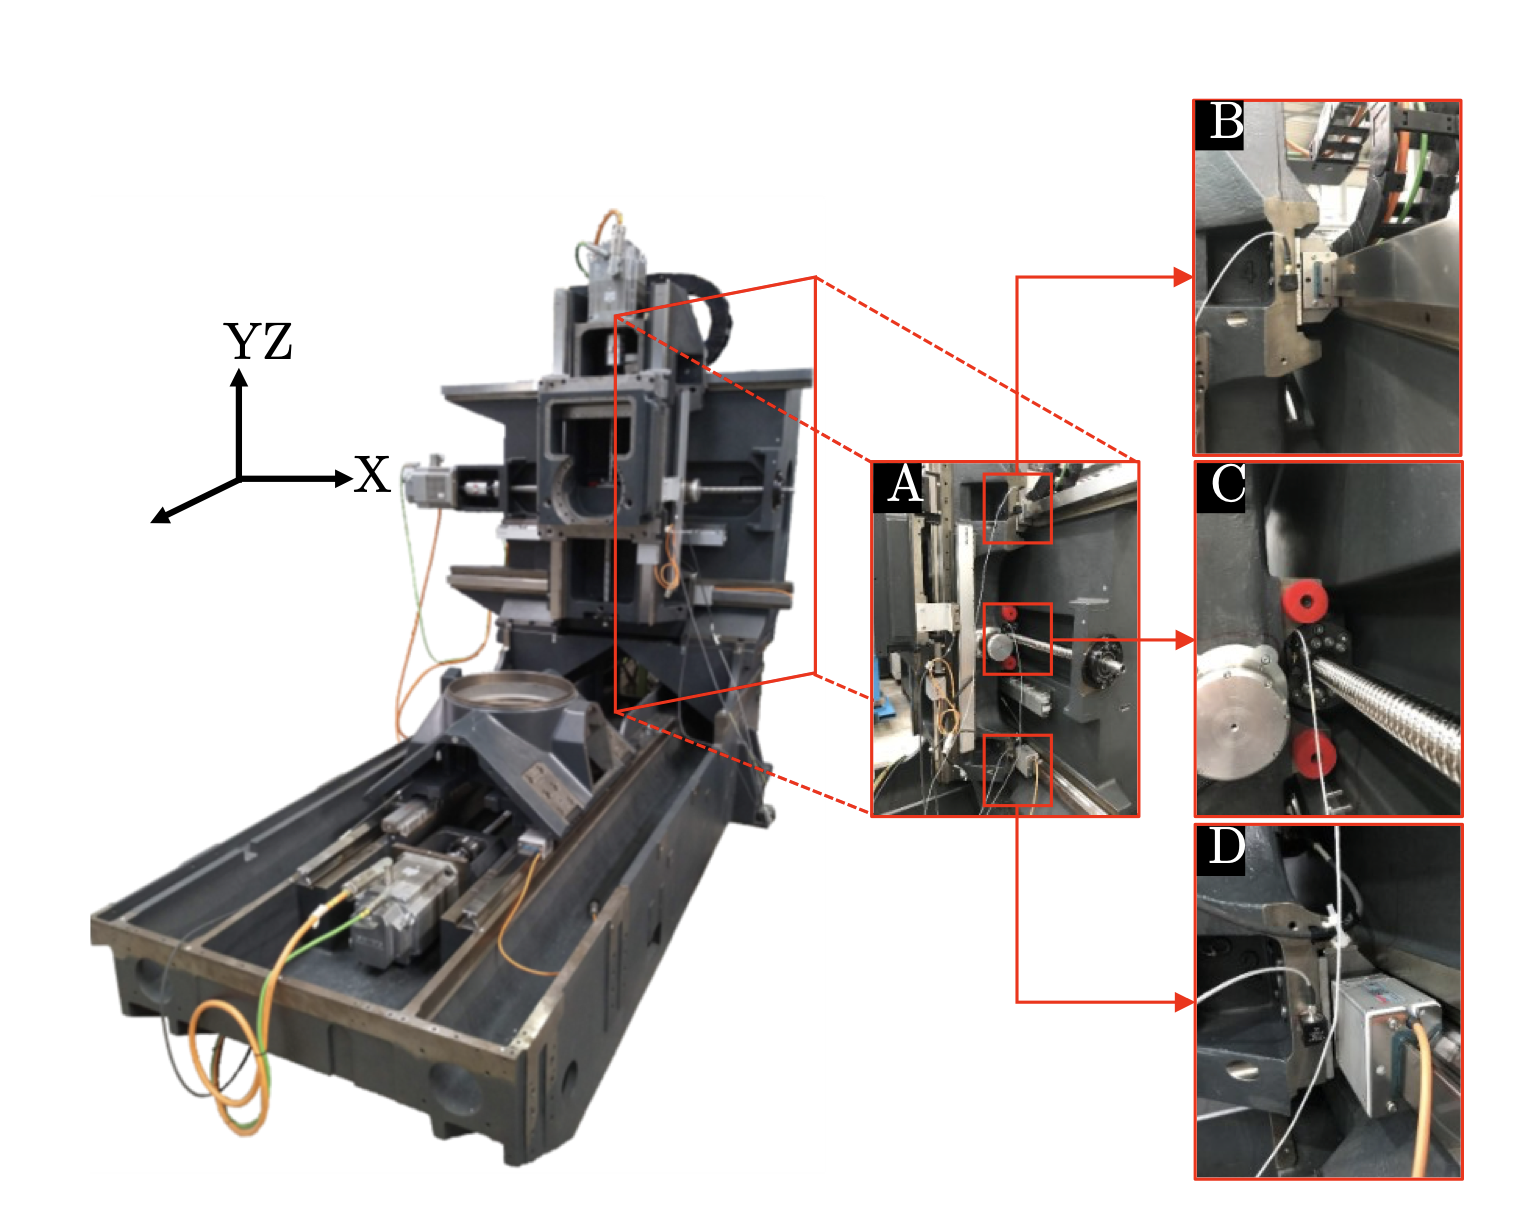
\includegraphics[width=0.9\textwidth]{experimental_setup}
  \caption {Experimental Setup: A: side-view of the machine, B: Upper LGS conterparts, C: threaded shaft of the BSD, C: Lower LGS conterparts}
  \label{fig:experimental_setup}
\end{figure}

The software tool TNC Scope uses an oscilloscope to provide internal control data. Three triaxial Kistler 8762A10 piezo-eletric accelerometers are mounted at different positions (bottom, nut, top) and track the accelerations in all spatial directions when moving the machine tool along the x-axis.

\section{Dataset: Ball Screw Drive}
For the sake of reproducibility, the experiments are executed with a defined test cycle, which is defined in fig. \ref{fig:test_cycle}. Machine data is collected during constant speed, direction change and sweep excitement along the machine tools X-axis. During the constant speed excitement, the machine tools are moved back and forth along the whole axis ($\Delta x$ = 600mm). During the direction change excitation, the movement of the machine tools is restricted to a small part of the axis ($\Delta x$ = 1mm) and the directions are changed with a high frequency. In the sweep excitement, the motor, moving the machine tools along the different axis, receives a target speed in the form of a sine sweep. Before recording data, the machine is warmed up to create equivalent circumstances for each run. A constant speed excitement is applied for 60 min. 

\begin{figure}[H]
  \centering
  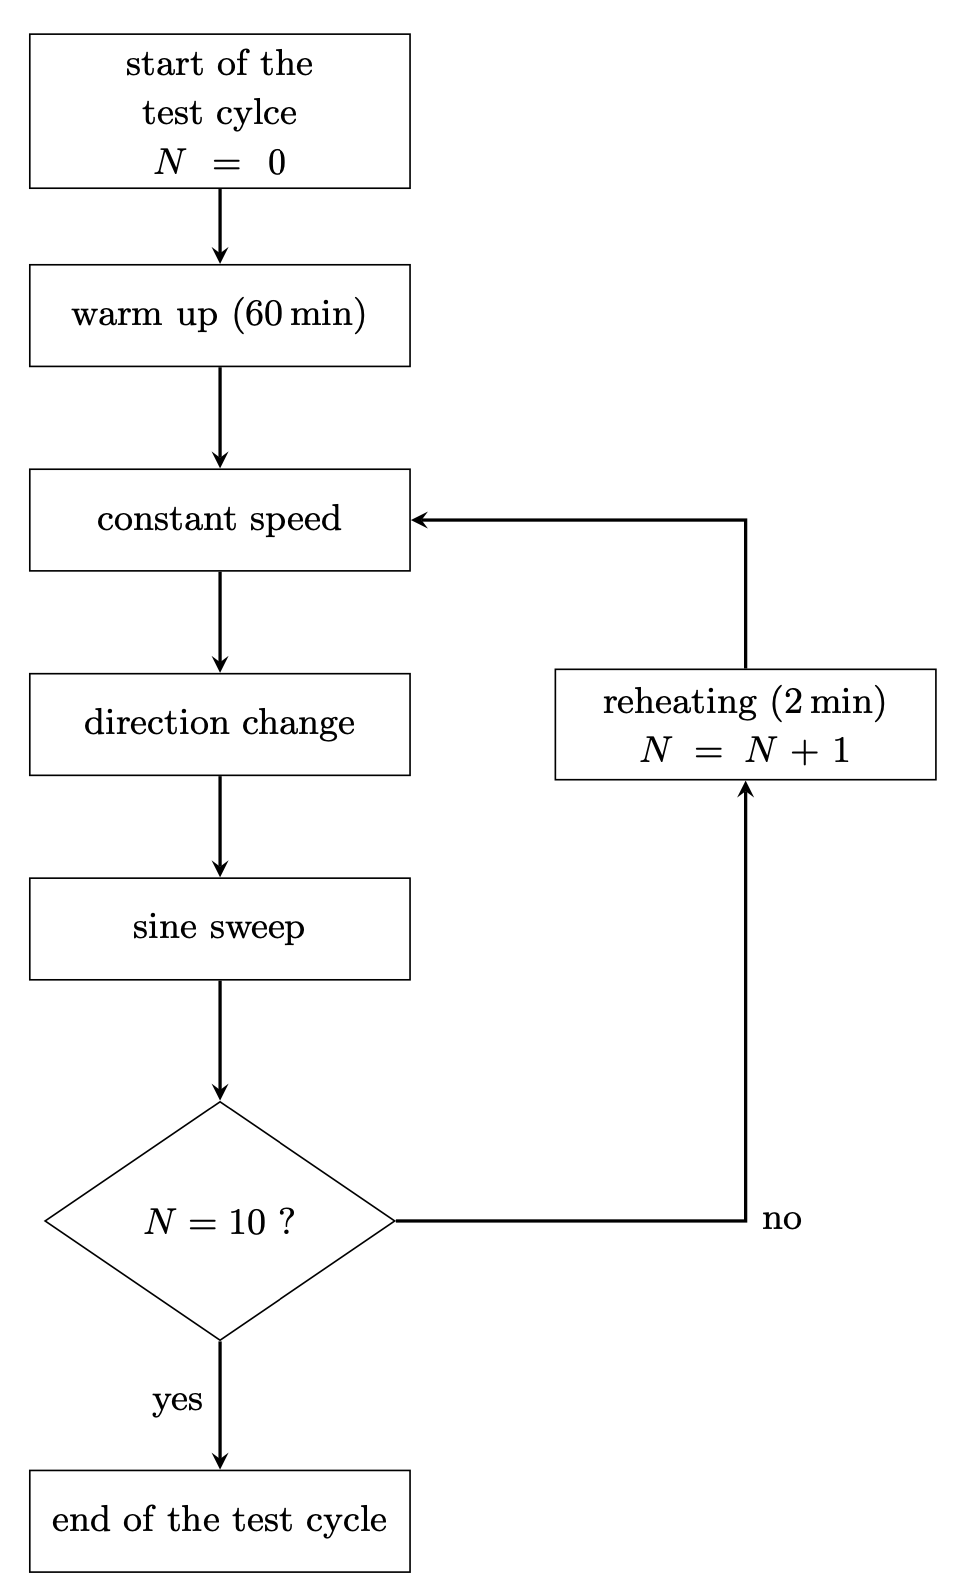
\includegraphics[width=0.7\textwidth]{test_cycle}
  \caption {Flow chart explaining the test cycle used in the presented dataset}
  \label{fig:test_cycle}
\end{figure}

In total 49 different signals are recorded during one sub cycle. The signals are specified in more detail in table. \ref{tab:description_of_the_49_recorded_features}. All feature names starting with "C" correspond to the constant speed , "D" to the direction change and "S" to the sweep excitement.

\begin{center}
\begin{longtable}{||c c c c||} 
 \hline
 name & sensor & frequency & samples \\ [0.5ex] 
 \hline\hline
 C:s ist/X & TNC Scope & 10 kHz & 75000 \\ 
 \hline
 C:s soll/X & TNC Scope & 10 kHz & 75000 \\ 
 \hline
 C:s diff/X & TNC Scope & 10 kHz & 75000 \\ 
 \hline
 C:v (n ist)/X & TNC Scope & 10 kHz & 75000 \\ 
 \hline
 C:v (n soll)/X& TNC Scope & 10 kHz & 75000 \\ 
 \hline
 C:P mech./X & TNC Scope & 10 kHz & 75000 \\ 
 \hline
 C:Pos. Diff./X & TNC Scope & 10 kHz & 75000 \\ 
 \hline
 C:I ist/X & TNC Scope & 10 kHz & 75000 \\ 
  \hline
 C:I soll/X & TNC Scope & 10 kHz & 75000 \\ 
 \hline
 C:x bottom & Acc & 10 kHz & 75000 \\ 
 \hline
 C:y bottom & Acc & 10 kHz & 75000 \\ 
 \hline
 C:z bottom & Acc & 10 kHz & 75000 \\ 
 \hline
 C:x nut & Acc & 10 kHz & 75000 \\ 
 \hline
 C:y nut & Acc & 10 kHz & 75000 \\ 
 \hline
 C:z nut & Acc & 10 kHz & 75000 \\ 
 \hline
  C:x top & Acc & 10 kHz & 75000 \\ 
 \hline
 C:y top & Acc & 10 kHz & 75000 \\ 
 \hline
 C:z top & Acc & 10 kHz & 75000 \\ 
 \hline
 D:s ist/X & TNC Scope & 10 kHz & 75000 \\
 \hline
 D:s soll/X & TNC Scope & 10 kHz & 75000 \\ 
 \hline
 D:s diff/X & TNC Scope & 10 kHz & 75000 \\ 
 \hline
 D:v (n ist)/X & TNC Scope & 10 kHz & 75000 \\ 
 \hline
 D:v (n soll)/X & TNC Scope & 10 kHz & 75000 \\ 
 \hline
 D:P mech./X & TNC Scope & 10 kHz & 75000 \\ 
 \hline
 D:Pos. Diff./X & TNC Scope & 10 kHz & 75000 \\ 
  \hline
 D:I ist/X & TNC Scope & 10 kHz & 75000 \\ 
 \hline
 D:I soll/X & TNC Scope & 10 kHz & 75000 \\ 
 \hline
 D:x bottom & Acc & 10 kHz & 75000 \\ 
  \hline
 D:y bottom & Acc & 10 kHz & 75000 \\ 
 \hline
 D:z bottom & Acc & 10 kHz & 75000 \\ 
 \hline
 D:x nut & Acc & 10 kHz & 75000 \\ 
 \hline
 D:y nut & Acc & 10 kHz & 75000 \\ 
 \hline
 D:z nut & Acc & 10 kHz & 75000 \\ 
 \hline
 D:x top & Acc & 10 kHz & 75000 \\
  \hline
 D:y top & Acc & 10 kHz & 75000 \\ 
 \hline
 D:z top & Acc & 10 kHz & 75000 \\ 
 \hline
 S:x bottom & Acc & 10 kHz & 153601 \\ 
 \hline
 S:y bottom & Acc & 10 kHz & 153601 \\ 
 \hline
 S:z bottom & Acc & 10 kHz & 153601 \\ 
 \hline
 S:x nut & Acc & 10 kHz & 153601 \\ 
  \hline
 S:y nut & Acc & 10 kHz & 153601 \\ 
 \hline
 S:z nut & Acc & 10 kHz & 153601 \\ 
 \hline
 S:x top & Acc & 10 kHz & 153601 \\ 
 \hline
 S:y top & Acc & 10 kHz & 153601 \\ 
 \hline
 S:z top & Acc & 10 kHz & 153601 \\ 
 \hline
 S:Nominal rotational speed & TNC opt & 1 kHz & 16384 \\
  \hline
 S:Actual rotational speed & TNC opt & 1 kHz & 16384 \\ 
 \hline
 S:Actual position of the position encoder(dy/dt) & TNC opt & 1 kHz & 16384 \\ 
 \hline
 S:Actual position of the motor encoder(dy/dt)  & TNC opt & 1 kHz & 16384  \\ [1ex] 
 \hline
\caption {feature description of the 49 different time-series}
\label {tab:description_of_the_49_recorded_features}
\end{longtable}
\end{center}

Due to abrasion, the different machine components wear down. LGSs are separated in three and the BSDs in four different health condition classes. Usually, the lifetime of BSDs is shorter than that of the LGSs. This means that ball screws need to be replaced in shorter internals. Different combinations of LGSs and BSDs health condition classes were recorded, which are shown in the following table. \ref{tab:recorded_combinations_of_LGS_and_BSD_health_conditions}

\begin{table}[ht]
  \large
  \centering
  \begin{tabular}{c|c||*{9}{c|}}
    \multicolumn{2}{c}{} & \multicolumn{9}{c}{BSD} \tabularnewline
    \cline{2-11}
    \multirow{5}*{\rotatebox{90}{LGS}} &
&    \bfseries C31 & \bfseries C21 & \bfseries C11 & \bfseries P1 & \bfseries C22 &\bfseries C12 & \bfseries C32 &\bfseries C33 &\bfseries P2  \tabularnewline[1 ex] 
\cline{2-11}
&    \bfseries C3 & 1 &  2 &  3 & 4 & 5 & 6 & 7 & 8 & 9 \tabularnewline [1ex] 
    \cline{2-11}
&    \bfseries C2 & 10 &  11 &  12 &  13 & 14 & 15 & 16 & 17 & 18\tabularnewline [1ex] 
    \cline{2-11}
&    \bfseries C1 & 18 & 19 & 20 & 21 & 23 & 24 & 25 & 26 & 27 \tabularnewline [1ex] 
    \cline{2-11}
  \end{tabular}
\caption {Recorded combinations of LGS and BSD health conditions}
\label {tab:recorded_combinations_of_LGS_and_BSD_health_conditions}
\end{table} 

For the experiments, two domains were defined. The source domain consists of the health condition states 2, 3, 11, 12, 20, 21 and the target domain of 5, 6, 14, 15, 23, 24. The model is trained to predict the health condition class of the BSD. Both the source and target domain includes the four BSD health condition classes C1, C2, C3 and P1 combined with all three LGS preload classes C1, C2, C3. In order to generate a binary classification problem, the BSD states C1 and P1 were combined as "healthy" and C2 and C3 as "degraded" class. The source and target domain includes the same combination of BSD and LGS health condition classes, just from two different observations (source: observation 1, target:observation 2). In both observations, the used LGSs are the exact same components, but Contrariwise, different BSD components with similar degradation levels were used. The defined health condition classes of the BSDs are defined differently for the two observations. Table \ref {tab:BSDs_states} shows that the defined preload for C11 and C12, C21 and C22, C31 and C32 as well as P1 and P2 differ with up to 147 N. This inhomogeneous definition of the BSD health condition classes as well as marginal differences in the production and installation of the BSDs leads to a significant domain shift problem, which affects the performance of the model during the testing enormously. 


\section{Dummy Dataset}
The applicability of different domain-adaption approaches in the context of PHM was evaluated on a synthetic dummy dataset, which is structured equally and shows similar patterns as the corresponding real-world dataset. The complexity of the data and therefore the task can be tuned arbitrarily. A dataset like that can help to understand underlying mechanisms of new and unknown approaches. Besides that, it serves as a prior evaluation for the approach's applicability for a given real-world task. In this work, a simple dummy dataset was established to evaluate the MMD loss to learn a more domain-invariant feature extraction. Since one has to deal with irregularities, outliers and noise in real-world data, it is helpful to evaluate the MMD loss on a dataset which is not disturbed by these effects. Similarly to PHM applications, the model in the dummy dataset processes time sequences. In the dummy example, the time sequences consist of 1000 data points which are sampled from a cosine  curve. The synthetic dataset which simulates the classification problem with two classes and two domains is sampled from four cosine  curves, each with characteristic amplitudes and frequencies. By adjusting the amplitude and frequency, the domain adaption problem can be configured more or less difficult. The sampling process must include a certain randomness to allow differing sequences for the same class and domain. For every sampling step, the domain- and class-specific amplitude and frequency of the cosine  curve is perturbed. This changes the underlying characteristic of each sequence. Besides that, noise is added to each of the 1000 data points within that sequence. This is necessary to generate a periodic signal which is close to a noisy real-world vibration signal. For the sake of simplicity, the dataset contains just 1-D sequences. This simulates a health monitoring task on just one single signal. In Fig. \ref{fig:samples_domain_class_dummy} four data sequences are shown representing one example sequence for each class and domain. 

\begin{figure}[H]
  \centering
  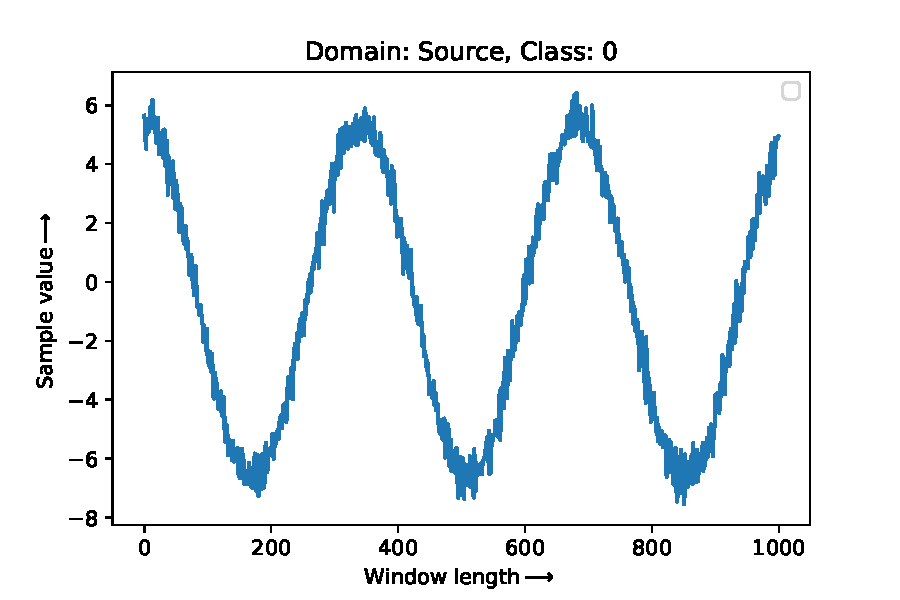
\includegraphics[width=.42\textwidth]{samples_domain_class_dummy/ex_dummy_source_class_0.pdf}
  \hspace{.3cm}
  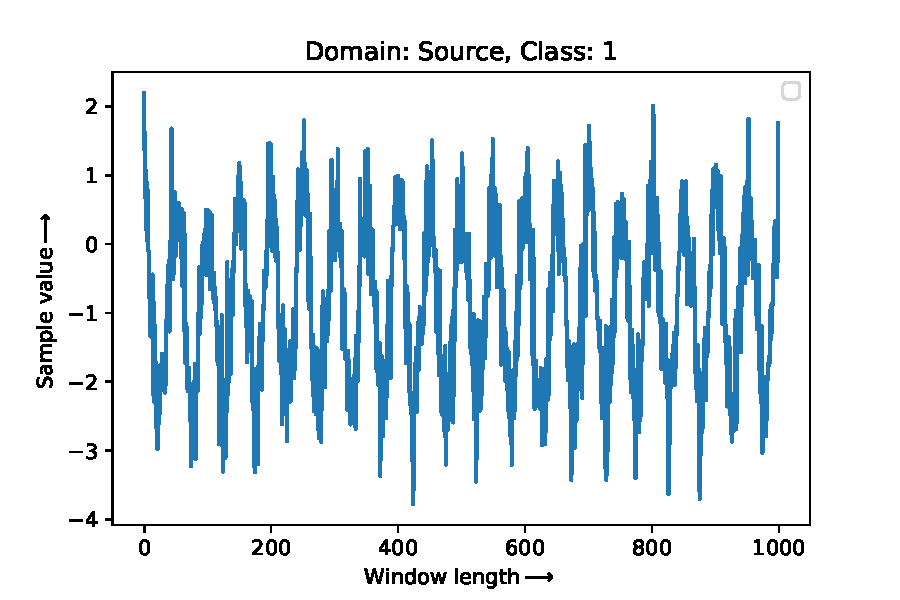
\includegraphics[width=.42\textwidth]{samples_domain_class_dummy/ex_dummy_source_class_1.pdf}

  \vspace{.1cm}

  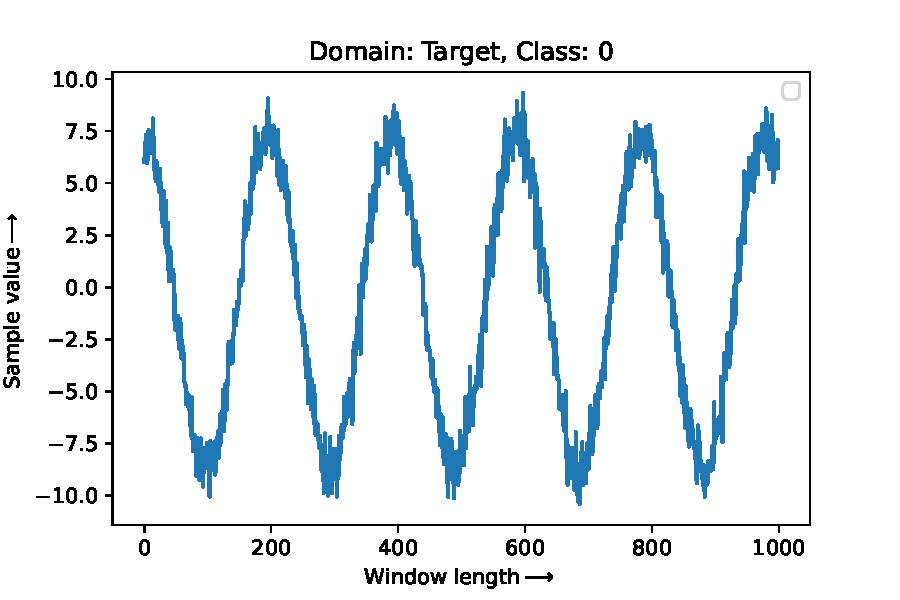
\includegraphics[width=.42\textwidth]{samples_domain_class_dummy/ex_dummy_target_class_0.pdf}
  \hspace{.3cm}
  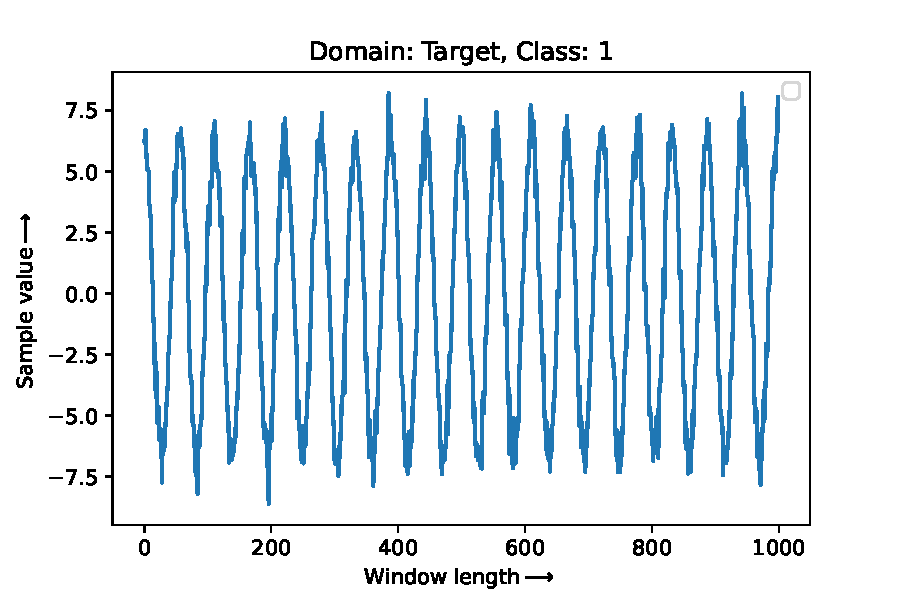
\includegraphics[width=.42\textwidth]{samples_domain_class_dummy/ex_dummy_target_class_1.pdf}

  \caption{Data Window Samples for each domain and class}
  \label{fig:samples_domain_class_dummy}
\end{figure}


In fig. \ref{fig:samples_domain_class_dummy_influence_noise} one can see how the applied perturbation and noise during the sampling process changes the data sequences belonging to the same class and domain. 


\begin{figure}[H]
  \centering
  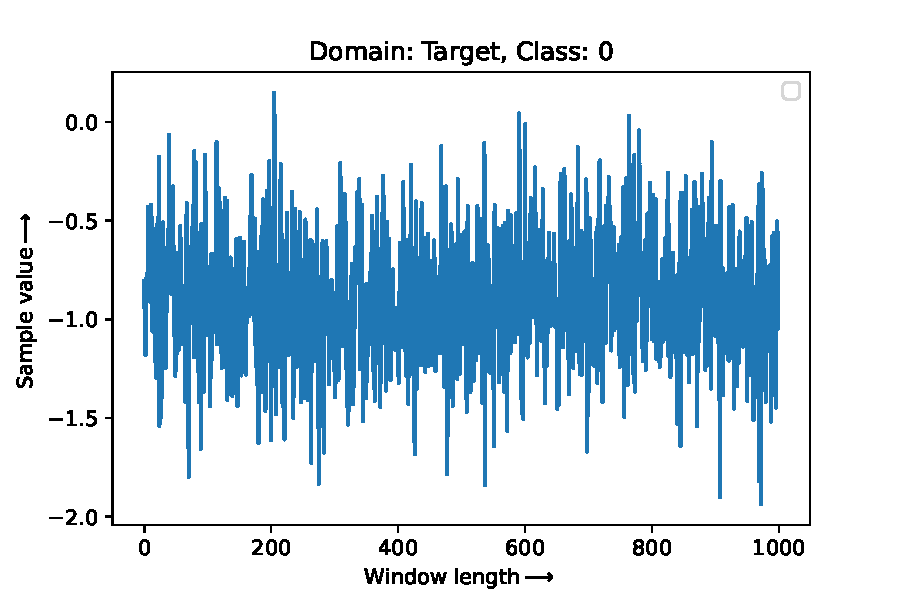
\includegraphics[width=.42\textwidth]{samples_domain_class_dummy_influence_noise/ex_dummy_target_class_0_ex_0.pdf}
  \hspace{.3cm}
  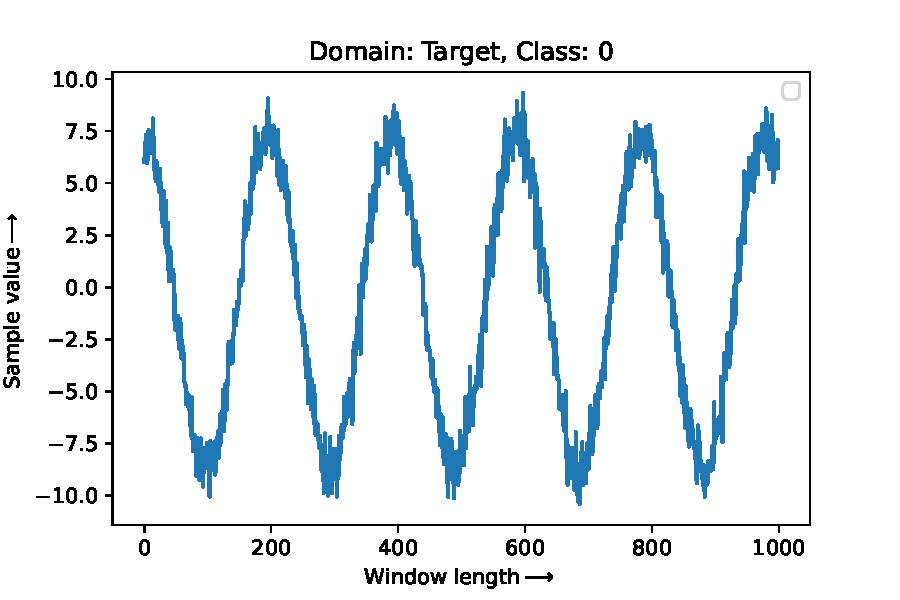
\includegraphics[width=.42\textwidth]{samples_domain_class_dummy_influence_noise/ex_dummy_target_class_0_ex_1.pdf}

  \vspace{.1cm}

  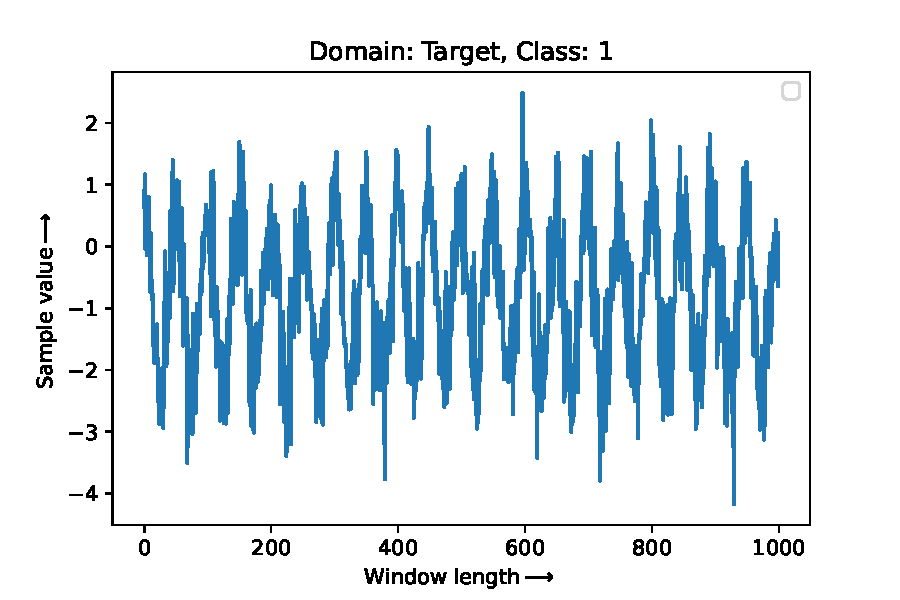
\includegraphics[width=.42\textwidth]{samples_domain_class_dummy_influence_noise/ex_dummy_target_class_1_ex_0.pdf}
  \hspace{.3cm}
  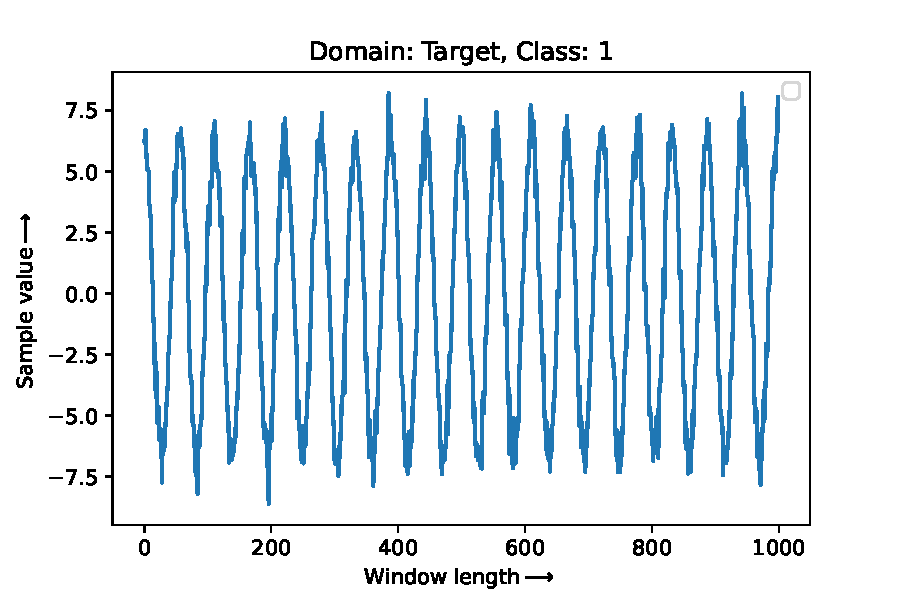
\includegraphics[width=.42\textwidth]{samples_domain_class_dummy_influence_noise/ex_dummy_target_class_1_ex_1.pdf}

  \caption{Influence of perturbation when sampling several data sequences for one class and domain}
  \label{fig:samples_domain_class_dummy_influence_noise}
\end{figure}



\section{Methods}\label{chapter:introduction}
In the following the model used in this thesis as well as the applied training concepts are presented

\subsection{Model}
\label{sec:model}
The model used during the experiments consists of a 1D CNN which is responsible to extract expressive features and a subsequent classifier predicting the health condition classes of the BSDs. A more detailed. visualization of the architecture is shown in fig.\ref{fig:proposed_model}. The CNN consists of 3 convolutional layers. With increasing network depth the spatial dimension of the feature map is decreased and its channel size increased. This helps to extract more global features in shallow and more specific and local features in deeper layers. The exact parameters of the convolutional layers are described in table \ref{tab:parameter_conv} 

\begin{longtable}{||c c c c||} 
\hline
& Conv 1 & Conv 2 & Conv 3 \\
\hline
kernel size & 100 & 10 & 5 \\
\hline
padding size & 0 & 1 & 1 \\
\hline
stride & 1 & 1 & 1 \\
\hline
\caption {Parameter convolutional layer}
\label {tab:parameter_conv}
\end{longtable}

Several pooling layers are included after the convolutional layers to reduce the spatial dimension of the feature maps. Reducing the model complexity prevents problems like overfitting and exploding gradients. Applying batch normalization after convolutional layers fixes the means and variances of the layers inputs for each batch, which helps to make the training faster and more stable. After iteratively applying these three types of layers the output of the CNN is flattened and normalized to a 1D vector. This vector is used as an input for the subsequent classifier. The latent feature space dimension of the classifier is reduced constantly. The two neurons in the output layer of the neural network represents the prediction probability for the two defined BSD health condition classes.


\begin{figure}[H]
  \centering
  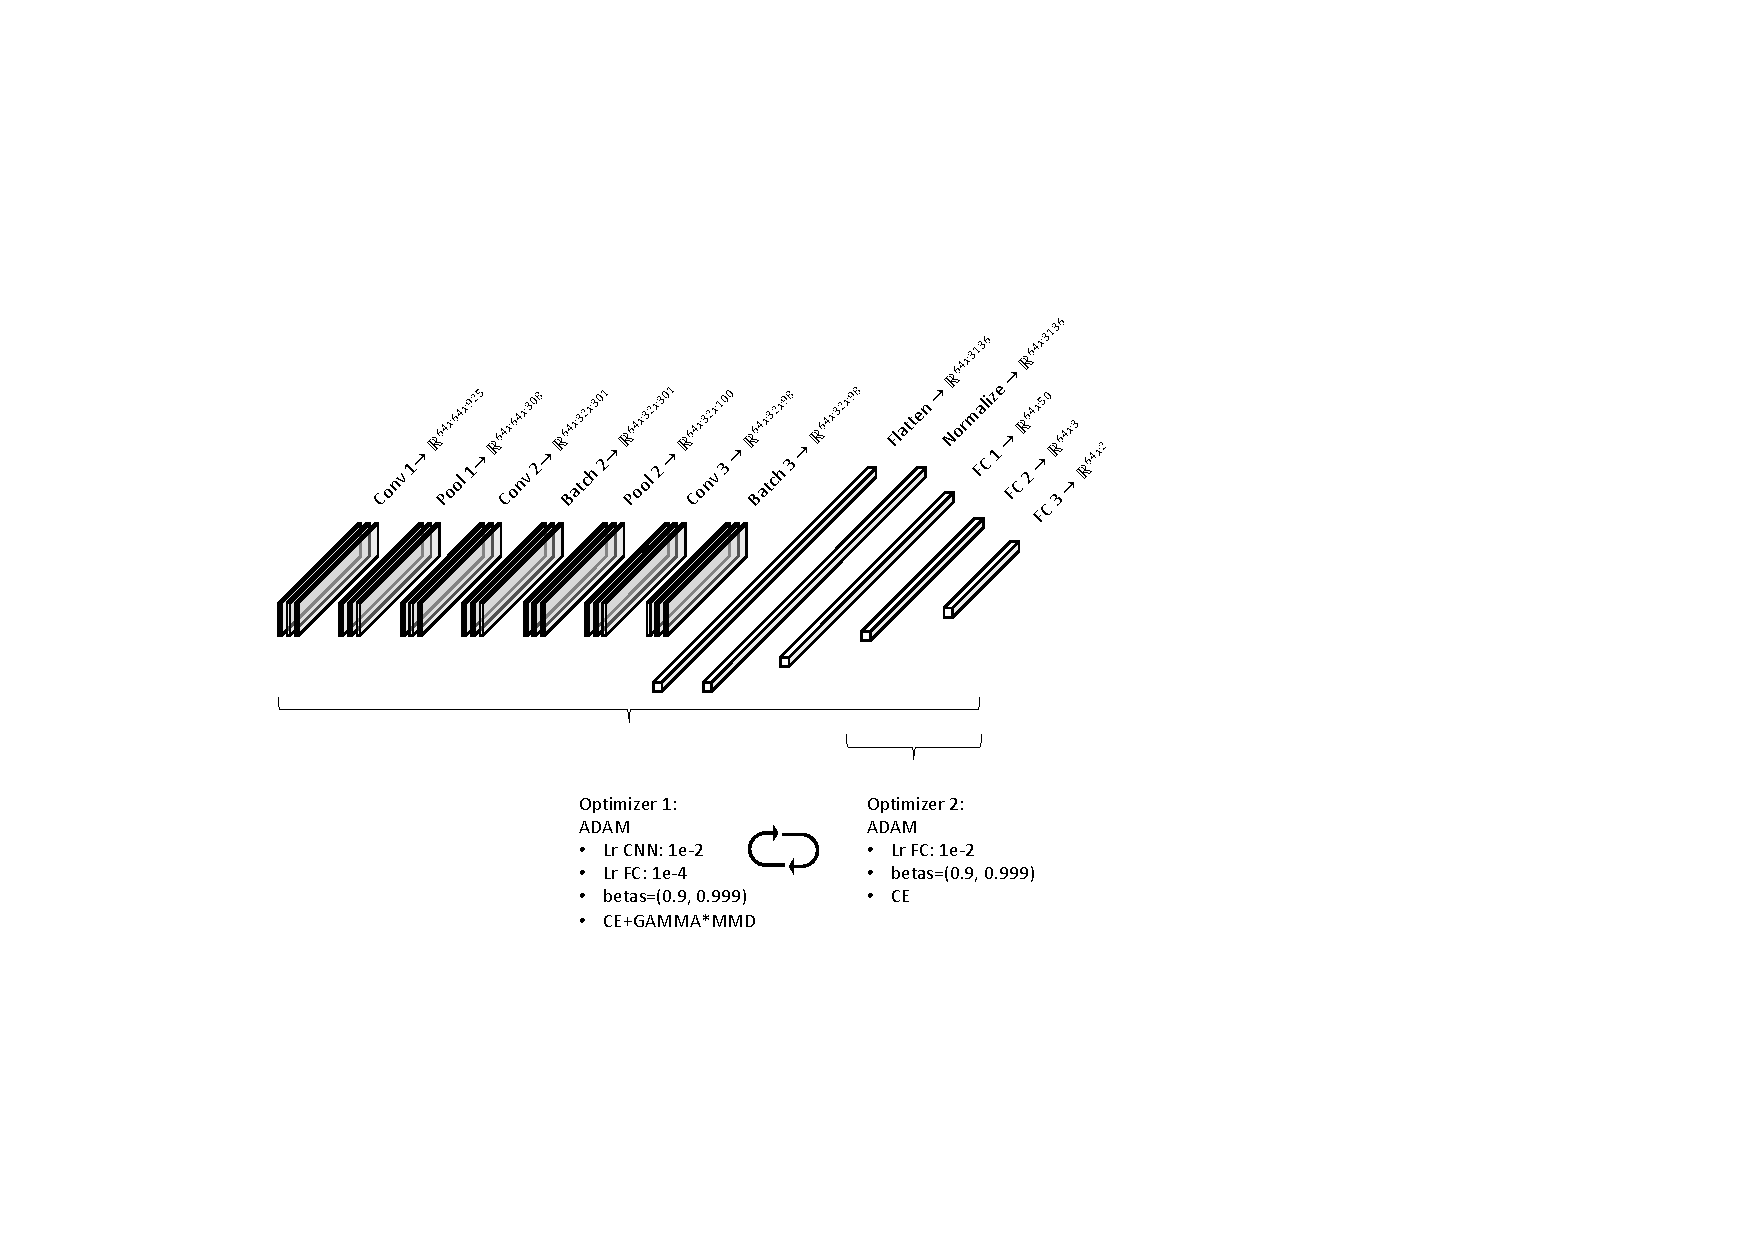
\includegraphics[width=1\textwidth]{proposed_model.pdf}
  \caption {Proposed model} \label{fig:proposed_model}
\end{figure}


\subsection{Proposed training with MMD and cross entropy loss} \label{sec:Proposed_training}

Firstly, the data used for the training is pre-processed. A dataloader is used to prepare the dataset. In a first step, the data is separated in shorter sequences of length 1024. These windows, which can include several of the recorded 49 signals, are fed as samples to the model. The sequences are cleaned from Nan values and synchronized afterwards. The dataset is randomly separated in a train, validation and test set with a split of 60\%/20\%/20\%. Also, the application of wavelet transforms, which can generate more informative data for the model, was partially investigated in this step. The repetitive training of the model is visualized in fig. \ref{fig:Training_Process_MMD}. A combination of a source cross-entropy and a MMD loss is applied to optimize the proposed deep-learning based domain adaption model. The MMD loss estimates the domain discrepancy in several latent feature maps. The MMD loss facilitates the extraction of more domain independent features within the model's layers. The cross entropy loss trains the model to increase the classification accuracy on the source domain. The domain discrepancy is measured as squared distance between distribution kernel embeddings in the reproducing kernel Hilbert space (RKHS). For the performance of the MMD loss, the kernel choice is of great importance. For this reason, several RBF kernels with bandwidth parameters 1, 2, 4, 8, 16 were combined in order to profit from their individual strength. For applying the MMD loss, two samples from each, source and target domain, are sampled randomly. For each such generated pair of samples, the MMD loss is calculated. The class of each sample is not considered in the MMD loss. Therefore, the MMD loss minimizes the domain discrepancy based on the observed source and target sample pairs, which partially belong to different but also to the same classes. The MMD is applied in several layers of the CNN and classifier. The source cross entropy loss is applied in the final layer. Fig. \ref{fig:MMD_Loss_and_CE_loss} symbolically shows how the MMD and the source cross-entropy loss is extracted from the different layers of the model.

\begin{figure}[H]
  \centering
  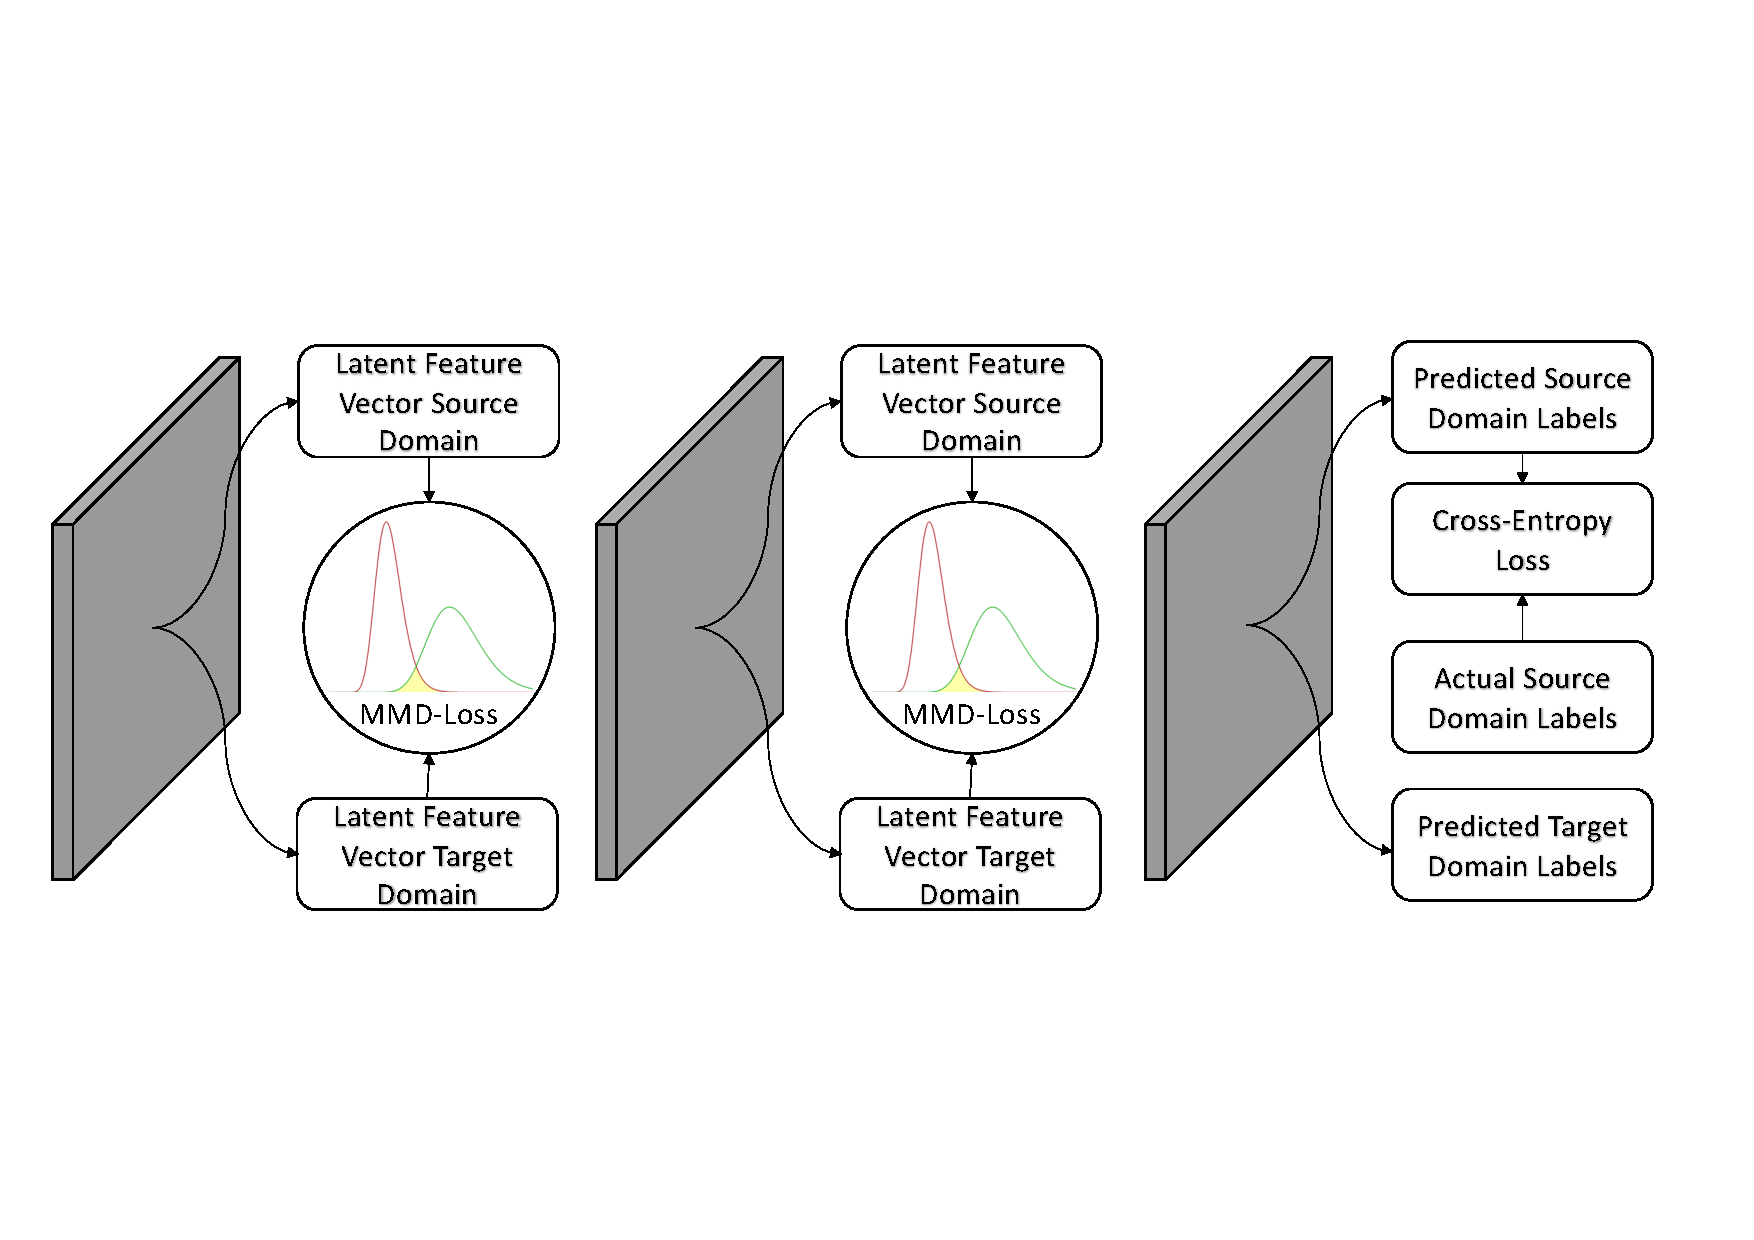
\includegraphics[width=1\textwidth]{MMD_loss_visualization.pdf}
  \caption {Cross Entropy Loss and MMD Loss in Neural Networks} \label{fig:MMD_Loss_and_CE_loss}
\end{figure}
 
A total loss must be specified by defining a weighted average between MMD and source cross entropy loss. The weighting factor GAMMA is a hyperparameter, which need to be defined beforehand. The total loss is defined as following:

\begin{align}
    \mbox{Total Loss} = \mbox{Source Cross-Entropy Loss} + \mbox{GAMMA} * \mbox{MMD Loss}
\end{align}.

The model training is separated in two phases. In a first phase, the Total Loss is applied on the whole network. An ADAM optimizer is used with different learning rates for the layers Conv1 to FC1 and FC2 to FC3. In a second phase, just the CE loss is applied to optimize the final two fully connected layers. Two-thirds of the train data is used in the first and one-third for the second train phase. The application of two different optimizer is visualized in fig. \ref{fig:proposed_model}. In general, the training is repeated until the maximum number of epochs is reached. After the training is completed, the model can be used to predict the BSD health condition state of unseen source and target domain samples. 

\begin{figure}[H]
  \centering
  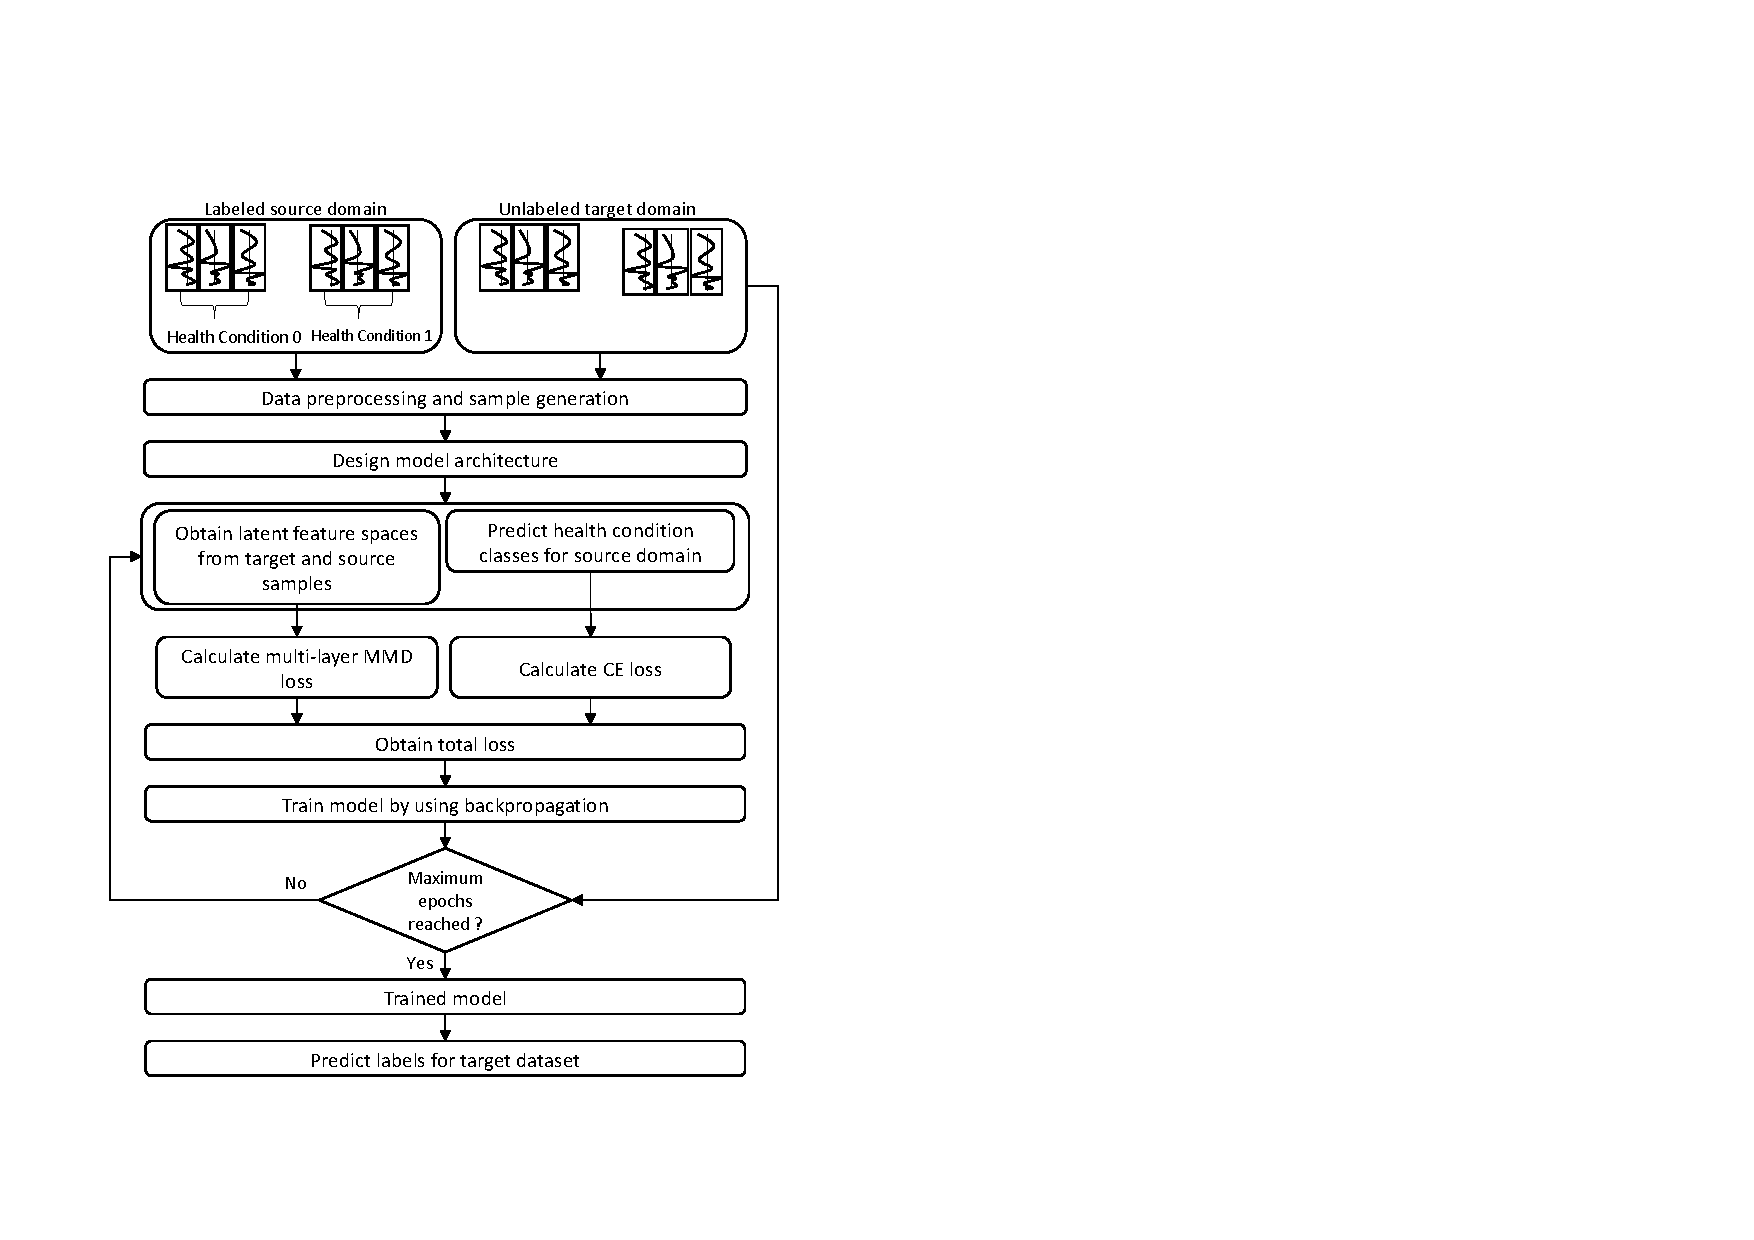
\includegraphics[width=0.8\textwidth]{training_process_mmd.pdf}
  \caption {Model training iteration} \label{fig:Training_Process_MMD}
\end{figure}

